\documentclass[usenatbib]{mnras}
\usepackage{graphicx}
\bibliographystyle{mnras}

\begin{document}

\begin{figure*}
  \centering
  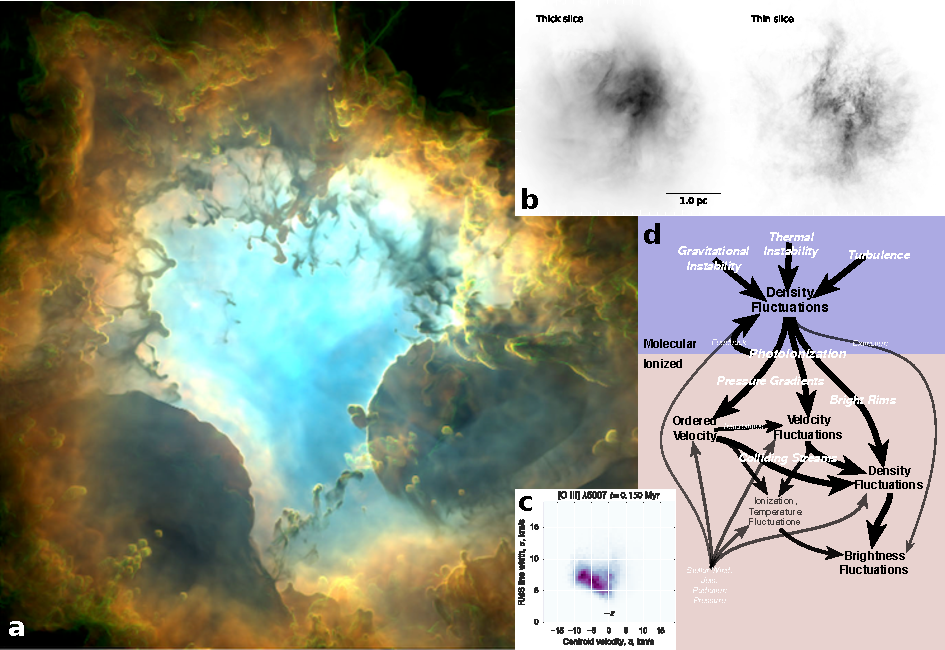
\includegraphics[width=\linewidth]{tom-review-arthur-henney}
  \caption{Turbulence in simulated H~II regions. (a) Simulated optical
    emission line image of H~II region at age of 250,000~years from
    \citet{Medina:2014a}, building on earlier work of
    \citet{Mellema:2006a, Arthur:2011a}. (b) Comparison of synthetic
    spectral maps using thick (left) versus thin (right) velocity
    slices.  The thick slice is sensitive only to emissivity
    fluctuations, whereas the thin slice is also sensitive to velocity
    fluctuations and therefore shows more fine-scale structure.  (c)
    Predicted joint distribution (PDF) of linewidth and centroid
    velocity for a simulated H~II region that shows a champagne flow
    towards the observer \citep{Arthur:2016a}.  (d) Causal
    relationships between different types of fluctuations in molecular
    clouds and H~II regions, as deduced from comparison between our
    synthetic observations and real observations of the Orion Nebula.
    Turbulence and ordered photoevaporation flows are found to
    contribute roughly equally to the observed density fluctuations.}
\end{figure*}

\bibliography{arthur-henney}


\end{document}

%%% Local Variables:
%%% mode: latex
%%% TeX-master: t
%%% End:
